\documentclass[10pt,a4paper]{article}
\usepackage[utf8]{inputenc}
\usepackage{graphicx}
\usepackage{url}
\title{Global Trends in Average Life Expectancy}
\author{AI Scientist evidence review}
\date{\today}
\begin{document}
\maketitle
\begin{abstract}
This evidence review surveys published literature and available public data on the stated topic. All plotted values come from the cited sources.
 Descriptive changes, extrema, and recent movement were calculated for 3 source-attributed time series.
\end{abstract}
\section{Introduction}
Research question: What are the primary global trends and regional disparities in average life expectancy over recent decades?. This report summarizes accessible published evidence.
\section{Search and data methods}
Searches were performed on 2026-09-30 using OpenAlex and Crossref with the following queries: global life expectancy trends temporal analysis; world mortality patterns life expectancy at birth; historical trends in human longevity global scale. Up to 30 deduplicated works were retained. Suggested World Bank and Our World in Data series were included only when the corresponding public API returned numerical observations. This is a targeted evidence review based on retrieved metadata and abstracts, not a full-text systematic review or a new experiment. For each validated series, compute the first-to-last net change, its average per elapsed calendar year, observed minimum and maximum, and changes between directly consecutive years. Report percentage change only for a positive starting value and nonnegative ending value. Compare the latest observation with the earliest available observation within the preceding five calendar years when this is a distinct interval. Missing years are not interpolated. These are descriptive statistics, not tests of significance or causation.
\section{Related literature}
The retrieved literature includes Global, regional, and national life expectancy, all-cause mortality, and cause-specific mortality for 249 causes of death, 1980-2015: a systematic analysis for the Global Burden of Disease Study 2015 [S1]. The retrieved literature includes Estimates and 25-year trends of the global burden of disease attributable to ambient air pollution: an analysis of data from the Global Burden of Diseases Study 2015 [S2]. The retrieved literature includes Global, regional, and national prevalence of overweight and obesity in children and adults during 1980-2013: a systematic analysis for the Global Burden of Disease Study 2013 [S3]. The retrieved literature includes Global, regional, and national incidence, prevalence, and years lived with disability for 354 diseases and injuries for 195 countries and territories, 1990-2017: a systematic analysis for the Global Burden of Disease Study 2017 [S4]. The retrieved literature includes Global and regional mortality from 235 causes of death for 20 age groups in 1990 and 2010: a systematic analysis for the Global Burden of Disease Study 2010 [S5]. The retrieved literature includes Global, regional, and national incidence, prevalence, and years lived with disability for 328 diseases and injuries for 195 countries, 1990-2016: a systematic analysis for the Global Burden of Disease Study 2016 [S6].
\section{Descriptive analysis of published data}
\subsection*{Life expectancy at birth, total (years) - World}
Life expectancy at birth, total (years) for World [D1] contains 25 observed values from 2000 to 2024. The value rose from 67.65 to 73.482 source-reported units, a net increase of 5.831 source-reported units. Relative to the starting value, this is a 8.62\% increase. The average net increase over the elapsed calendar years is 0.243 source-reported units per year. Among the observed points, the minimum is 67.65 in 2000 and the maximum is 73.482 in 2024. Across 24 directly consecutive-year pairs, 22 increased, 2 decreased, and 0 were unchanged. The latest available five-year window (2019-2024) shows a net increase of 0.6119 source-reported units.
\subsection*{Life expectancy at birth, female (years) - World}
Life expectancy at birth, female (years) for World [D2] contains 25 observed values from 2000 to 2024. The value rose from 70.09 to 75.973 source-reported units, a net increase of 5.883 source-reported units. Relative to the starting value, this is a 8.39\% increase. The average net increase over the elapsed calendar years is 0.2451 source-reported units per year. Among the observed points, the minimum is 70.09 in 2000 and the maximum is 75.973 in 2024. Across 24 directly consecutive-year pairs, 22 increased, 2 decreased, and 0 were unchanged. The latest available five-year window (2019-2024) shows a net increase of 0.6228 source-reported units.
\subsection*{Life expectancy - World}
Life expectancy for World [D3] contains 81 observed values from 1770 to 2023. The value rose from 28.5 to 73.169 source-reported units, a net increase of 44.669 source-reported units. Relative to the starting value, this is a 156.73\% increase. The average net increase over the elapsed calendar years is 0.1766 source-reported units per year. Among the observed points, the minimum is 28.5 in 1770 and the maximum is 73.169 in 2023. Across 73 directly consecutive-year pairs, 66 increased, 7 decreased, and 0 were unchanged. The latest available five-year window (2018-2023) shows a net increase of 0.7809 source-reported units.
\section{Figures}
\begin{figure}[htbp]
\centering
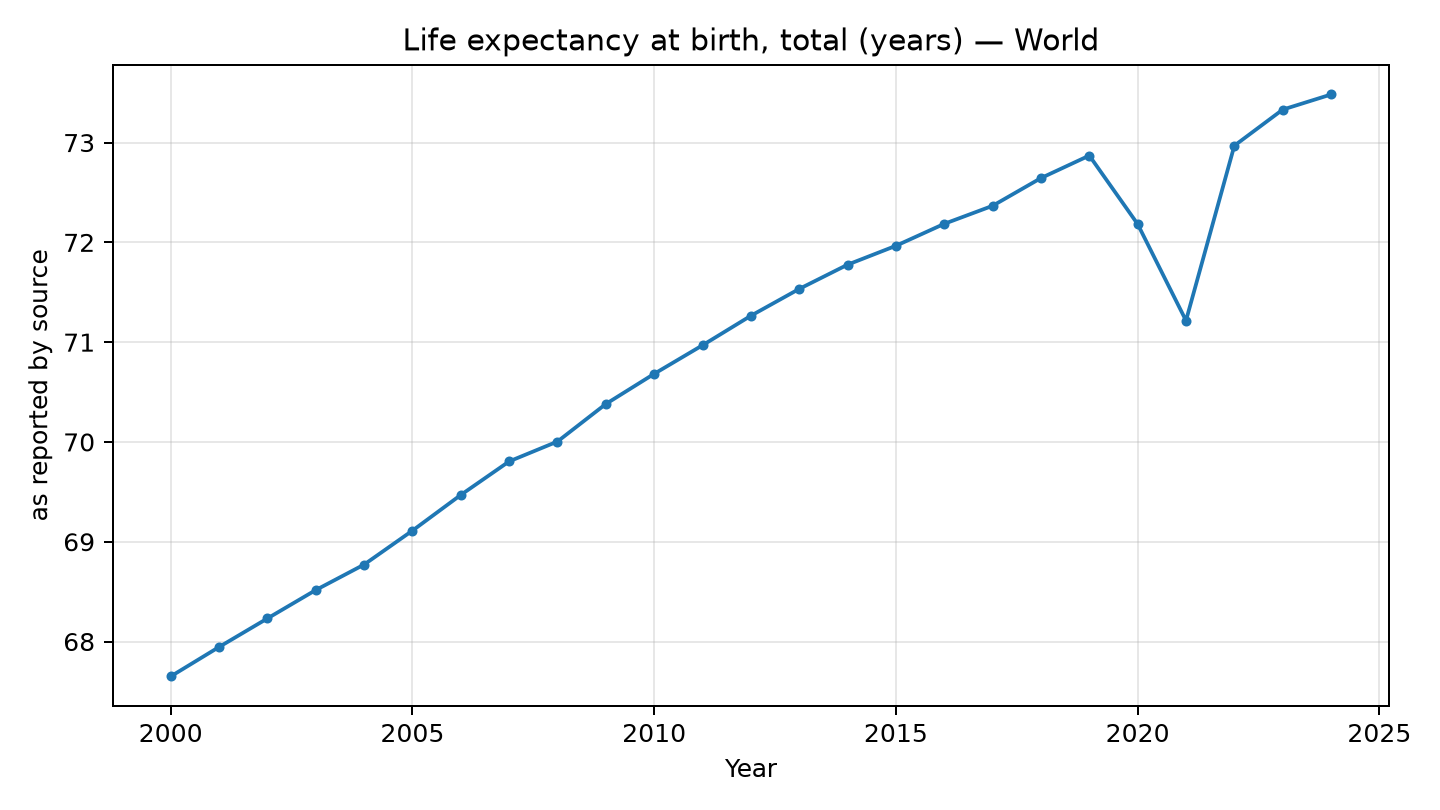
\includegraphics[width=0.85\linewidth]{chart_01.png}
\caption{Published values for World: Life expectancy at birth, total (years) (D1).}
\label{fig:chart1}
\end{figure}
\begin{figure}[htbp]
\centering
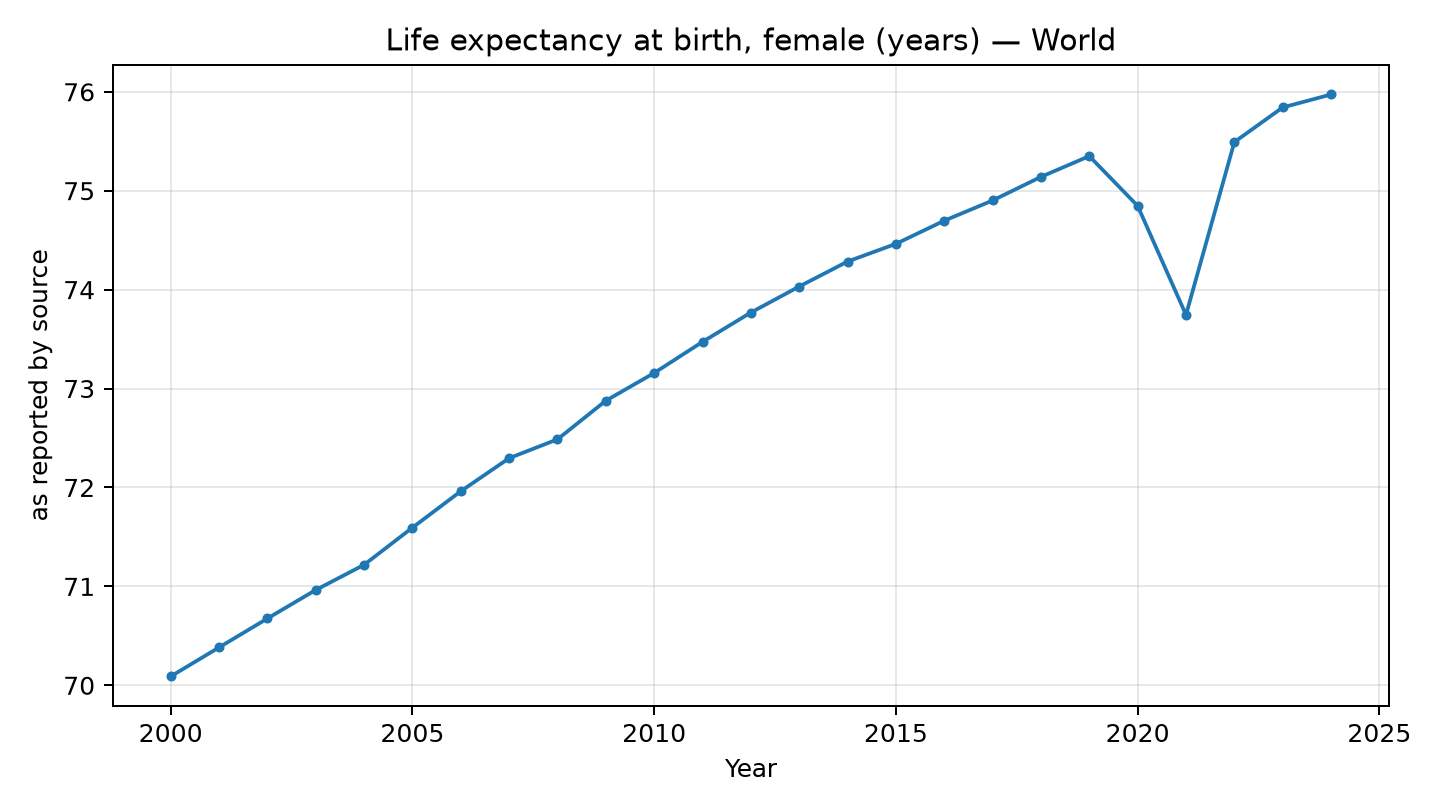
\includegraphics[width=0.85\linewidth]{chart_02.png}
\caption{Published values for World: Life expectancy at birth, female (years) (D2).}
\label{fig:chart2}
\end{figure}
\begin{figure}[htbp]
\centering
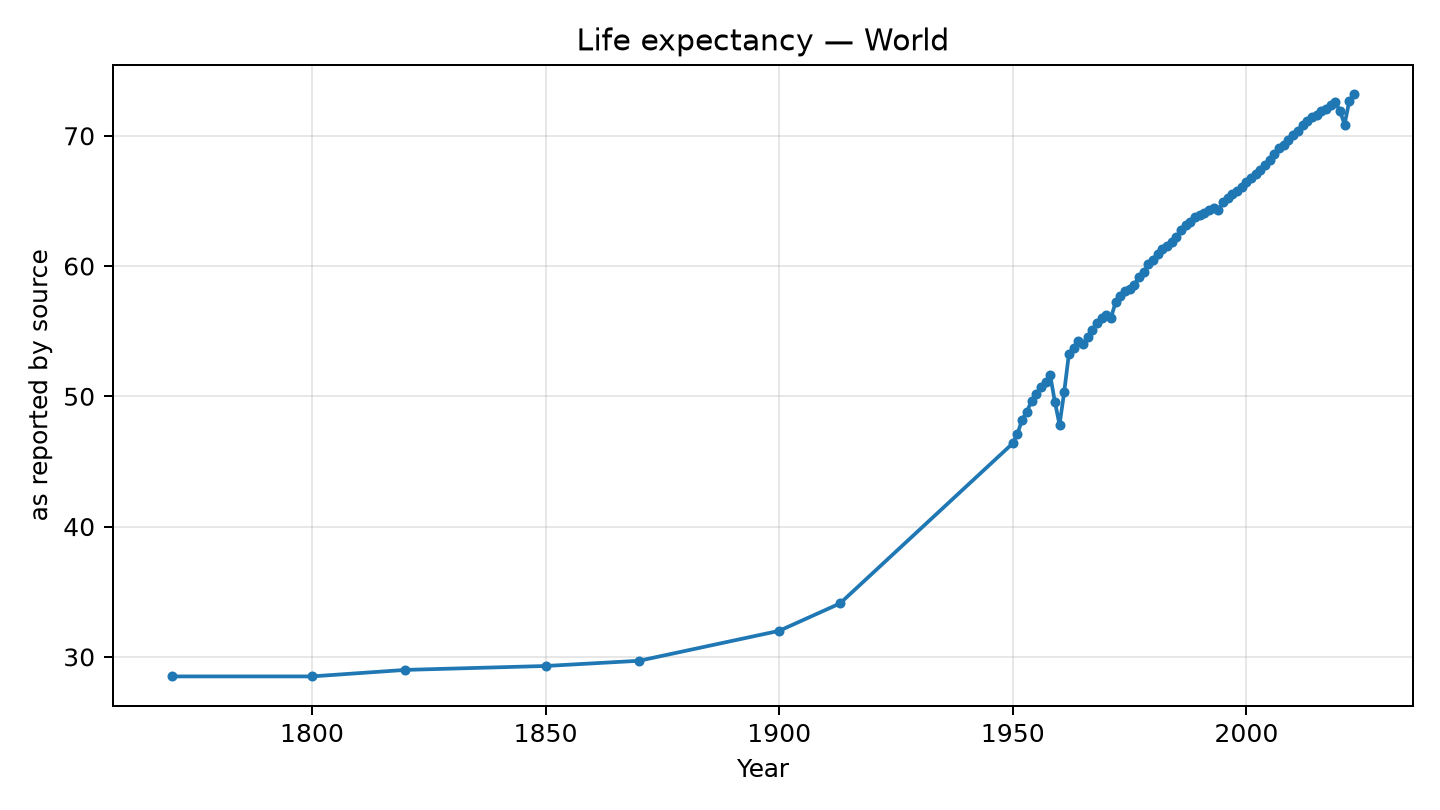
\includegraphics[width=0.85\linewidth]{chart_03.png}
\caption{Published values for World: Life expectancy (D3).}
\label{fig:chart3}
\end{figure}
\begin{figure}[htbp]
\centering
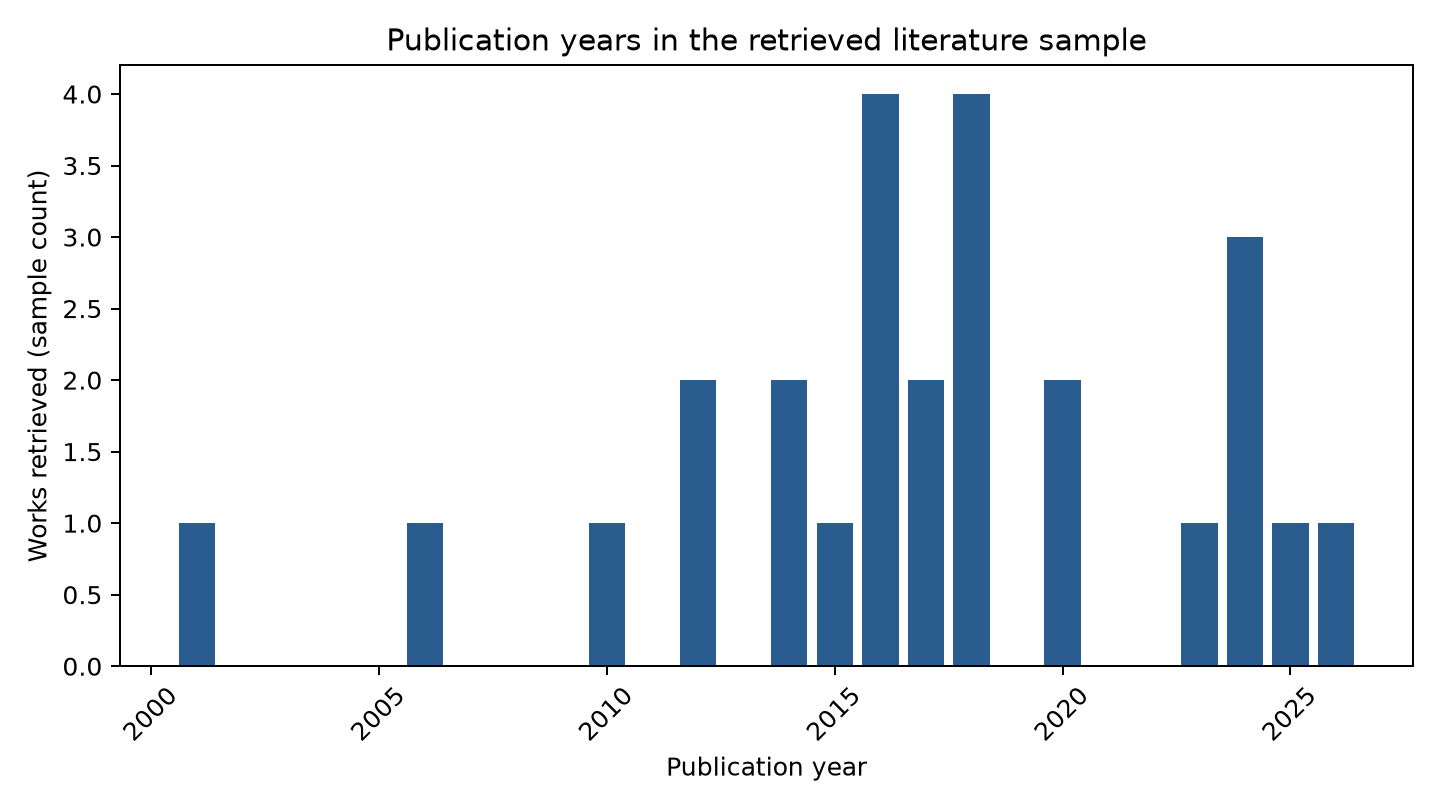
\includegraphics[width=0.85\linewidth]{chart_04.png}
\caption{Publication years of works retrieved from OpenAlex/Crossref; this search sample does not measure the topic's real-world outcome.}
\label{fig:chart4}
\end{figure}
\section{Discussion and limitations}
The quantitative findings are descriptive within each series. Changes in definitions, coverage, revisions, uncertainty, and missing years were not independently evaluated. Values from different providers should not be treated as directly comparable without checking their methods. No causal or statistical-significance claim follows from these summaries.
The selected sources differ in scope and coverage. The figures describe only the retrieved data and cannot establish causation.
\section{Conclusion}
Further interpretation requires review of the underlying sources and their methods.
\section*{References}
\noindent\textbf{[S1]} Haidong Wang, Mohsen Naghavi, Christine Allen, Ryan M Barber, Zulfiqar Ahmed Bhutta, Austin Carter, et al. (2016). Global, regional, and national life expectancy, all-cause mortality, and cause-specific mortality for 249 causes of death, 1980-2015: a systematic analysis for the Global Burden of Disease Study 2015. The Lancet. \url{https://doi.org/10.1016/s0140-6736(16)31012-1}\par

\noindent\textbf{[S2]} Aaron J. Cohen, Michael D Brauer, Richard Burnett, H Ross Anderson, Joseph Jon Frostad, Kara Estep, et al. (2017). Estimates and 25-year trends of the global burden of disease attributable to ambient air pollution: an analysis of data from the Global Burden of Diseases Study 2015. The Lancet. \url{https://doi.org/10.1016/s0140-6736(17)30505-6}\par

\noindent\textbf{[S3]} Marie Ng, Tom Fleming, Margaret Robinson, Blake Thomson, Nicholas Graetz, Christopher Margono, et al. (2014). Global, regional, and national prevalence of overweight and obesity in children and adults during 1980-2013: a systematic analysis for the Global Burden of Disease Study 2013. The Lancet. \url{https://doi.org/10.1016/s0140-6736(14)60460-8}\par

\noindent\textbf{[S4]} Spencer Lewis James, Degu Abate, Kalkidan Hassen Abate, Solomon Mequanente Abay, Cristiana Abbafati, Nooshin Abbasi, et al. (2018). Global, regional, and national incidence, prevalence, and years lived with disability for 354 diseases and injuries for 195 countries and territories, 1990-2017: a systematic analysis for the Global Burden of Disease Study 2017. The Lancet. \url{https://doi.org/10.1016/s0140-6736(18)32279-7}\par

\noindent\textbf{[S5]} Rafael Lozano, Mohsen Naghavi, Kyle J Foreman, Stephen S Lim, Kenji Shibuya, Victor Aboyans, et al. (2012). Global and regional mortality from 235 causes of death for 20 age groups in 1990 and 2010: a systematic analysis for the Global Burden of Disease Study 2010. The Lancet. \url{https://doi.org/10.1016/s0140-6736(12)61728-0}\par

\noindent\textbf{[S6]} Theo Vos, Amanuel Alemu Abajobir, Kalkidan Hassen Abate, Cristiana Abbafati, Kaja Abbas, Foad Abd-Allah, et al. (2017). Global, regional, and national incidence, prevalence, and years lived with disability for 328 diseases and injuries for 195 countries, 1990-2016: a systematic analysis for the Global Burden of Disease Study 2016. The Lancet. \url{https://doi.org/10.1016/s0140-6736(17)32154-2}\par

\noindent\textbf{[S7]} GBD 2023 Causes of Death Collaborators (2014). Global, regional, and national age-sex specific all-cause and cause-specific mortality for 240 causes of death, 1990-2013: a systematic analysis for the Global Burden of Disease Study 2013. The Lancet. \url{https://doi.org/10.1016/s0140-6736(14)61682-2}\par

\noindent\textbf{[S8]} Freddie Bray, Mathieu Laversanne, Hyuna Sung, Jacques Ferlay, Rebecca L. Siegel, Isabelle Soerjomataram, et al. (2024). Global cancer statistics 2022: GLOBOCAN estimates of incidence and mortality worldwide for 36 cancers in 185 countries. CA A Cancer Journal for Clinicians. \url{https://doi.org/10.3322/caac.21834}\par

\noindent\textbf{[S9]} Mohsen Naghavi, Kanyin Liane Ong, Amirali Aali, Hazim Ababneh, Yohannes Habtegiorgis Abate, Cristiana Abbafati, et al. (2024). Global burden of 288 causes of death and life expectancy decomposition in 204 countries and territories and 811 subnational locations, 1990-2021: a systematic analysis for the Global Burden of Disease Study 2021. The Lancet. \url{https://doi.org/10.1016/s0140-6736(24)00367-2}\par

\noindent\textbf{[S10]} Nicholas J Kassebaum, Megha Kataria Arora, Ryan M Barber, Zulfiqar Ahmed Bhutta, Jonathan Brown, Austin Carter, et al. (2016). Global, regional, and national disability-adjusted life-years (DALYs) for 315 diseases and injuries and healthy life expectancy (HALE), 1990-2015: a systematic analysis for the Global Burden of Disease Study 2015. The Lancet. \url{https://doi.org/10.1016/s0140-6736(16)31460-x}\par

\noindent\textbf{[S11]} Gregory A. Roth, George A. Mensah, Catherine Owens Johnson, Giovanni Addolorato, Enrico Ammirati, Larry M. Baddour, et al. (2020). Global Burden of Cardiovascular Diseases and Risk Factors, 1990-2019. Journal of the American College of Cardiology. \url{https://doi.org/10.1016/j.jacc.2020.11.010}\par

\noindent\textbf{[S12]} Colin Douglas Mathers, Dejan Loncar (2006). Projections of Global Mortality and Burden of Disease from 2002 to 2030. PLoS Medicine. \url{https://doi.org/10.1371/journal.pmed.0030442}\par

\noindent\textbf{[S13]} Theo Vos, Christine Allen, Megha Kataria Arora, Ryan M Barber, Zulfiqar Ahmed Bhutta, Alexandria Brown, et al. (2016). Global, regional, and national incidence, prevalence, and years lived with disability for 310 diseases and injuries, 1990-2015: a systematic analysis for the Global Burden of Disease Study 2015. The Lancet. \url{https://doi.org/10.1016/s0140-6736(16)31678-6}\par

\noindent\textbf{[S14]} Ahmedin Jemal, Carol E. Desantis, Elizabeth Ward (2010). Global Patterns of Cancer Incidence and Mortality Rates and Trends. Cancer Epidemiology Biomarkers \& Prevention. \url{https://doi.org/10.1158/1055-9965.epi-10-0437}\par

\noindent\textbf{[S15]} Mohammad Hossein Forouzanfar, Ashkan Afshin, Lily Alexander, H Ross Anderson, Zulfiqar Ahmed Bhutta, Stan Biryukov, et al. (2016). Global, regional, and national comparative risk assessment of 79 behavioural, environmental and occupational, and metabolic risks or clusters of risks, 1990-2015: a systematic analysis for the Global Burden of Disease Study 2015. The Lancet. \url{https://doi.org/10.1016/s0140-6736(16)31679-8}\par

\noindent\textbf{[S16]} Kyle J Foreman, Neal Marquez, Andrew J. Dolgert, Kai Glenn Fukutaki, Nancy Fullman, Madeline McGaughey, et al. (2018). Forecasting life expectancy, years of life lost, and all-cause and cause-specific mortality for 250 causes of death: reference and alternative scenarios for 2016-40 for 195 countries and territories. The Lancet. \url{https://doi.org/10.1016/s0140-6736(18)31694-5}\par

\noindent\textbf{[S17]} Haidong Wang, Kaja Abbas, Mitra Abbasifard, Mohsen AbbasiKangevari, Hedayat Abbastabar, Foad Abd-Allah, et al. (2020). Global age-sex-specific fertility, mortality, healthy life expectancy (HALE), and population estimates in 204 countries and territories, 1950-2019: a comprehensive demographic analysis for the Global Burden of Disease Study 2019. The Lancet. \url{https://doi.org/10.1016/s0140-6736(20)30977-6}\par

\noindent\textbf{[S18]} Theo Vos, Abraham D Flaxman, Mohsen Naghavi, Rafael Lozano, Catherine Michaud, Majid Ezzati, et al. (2012). Years lived with disability (YLDs) for 1160 sequelae of 289 diseases and injuries 1990-2010: a systematic analysis for the Global Burden of Disease Study 2010. The Lancet. \url{https://doi.org/10.1016/s0140-6736(12)61729-2}\par

\noindent\textbf{[S19]} Daniel Dicker, Grant Nguyen, Degu Abate, Kalkidan Hassen Abate, Solomon Mequanente Abay, Cristiana Abbafati, et al. (2018). Global, regional, and national age-sex-specific mortality and life expectancy, 1950-2017: a systematic analysis for the Global Burden of Disease Study 2017. The Lancet. \url{https://doi.org/10.1016/s0140-6736(18)31891-9}\par

\noindent\textbf{[S20]} E. Ray Dorsey, Alexis Elbaz, Emma L. Nichols, Nooshin Abbasi, Foad Abd-Allah, Ahmed Abdelalim, et al. (2018). Global, regional, and national burden of Parkinson's disease, 1990-2016: a systematic analysis for the Global Burden of Disease Study 2016. The Lancet Neurology. \url{https://doi.org/10.1016/s1474-4422(18)30295-3}\par

\noindent\textbf{[S21]} Emmanuelle Cambois, Geraldine Duthe, France Mesle (2023). Global Trends in Life Expectancy and Healthy Life Expectancy. Oxford Research Encyclopedia of Global Public Health. \url{https://doi.org/10.1093/acrefore/9780190632366.013.384}\par

\noindent\textbf{[S22]} 3.2. Trends in life expectancy, 1960-2006. \url{https://doi.org/10.1787/488117545007}\par

\noindent\textbf{[S23]} (2001). Introduction: A Global Revolution in Life Expectancy. Rising Life Expectancy. \url{https://doi.org/10.1017/cbo9781316036495.002}\par

\noindent\textbf{[S24]} David Walsh, Gerry McCartney (2024). What else is relevant for understanding the changed life expectancy trends?. Social Murder?. \url{https://doi.org/10.1332/policypress/9781447373070.003.0012}\par

\noindent\textbf{[S25]} Life Expectancy. PsycEXTRA Dataset. \url{https://doi.org/10.1037/e312252005-001}\par

\noindent\textbf{[S26]} Figure 3.2. Trends in life expectancy, 2005-16. \url{https://doi.org/10.1787/888933834300}\par

\noindent\textbf{[S27]} Emma Rath. Exploring the Determinants of Life Expectancy at Birth: Predicting and Forecasting Global Health Trends Using Statistical, Machine Learning, and Deep Learning Models.. \url{https://doi.org/10.63227/652.299.100}\par

\noindent\textbf{[S28]} Xuelin Cheng, Wenchang Jia, Jing Zhou, Yaxin Xu, Jian Zou, Ming Liu, et al. (2025). Changes and trends in mortality, disability-adjusted life years, life expectancy, and healthy life expectancy in China from 1990 to 2021: a secondary analysis of the global burden of disease 2021. Archives of Public Health. \url{https://doi.org/10.1186/s13690-025-01558-8}\par

\noindent\textbf{[S29]} Maria Nyolcas (2026). Exploring Life Expectancy Trends in Europe: An Exploratory Data Analysis Using World Health Organization (WHO) Data. \url{https://doi.org/10.2139/ssrn.6136291}\par

\noindent\textbf{[S30]} Matthias Egger, Leigh F Johnson (2015). Estimating trends in life expectancy in HIV-positive individuals. The Lancet Global Health. \url{https://doi.org/10.1016/s2214-109x(14)70383-3}\par

\noindent\textbf{[D1]} World Bank: Life expectancy at birth, total (years) (World). Credit: World Population Prospects, United Nations (UN), uri: UN Population Division;
Statistical databases and publications from national statistical offices, National Statistical Offices (NSOs), note: Derived from male and female life expectancy at birth from sources such as statistical databases and publications from national statistical offices.;
Demographic Statistics, Eurostat (ESTAT), note: Derived from male and female life expectancy at birth from sources such as Eurostat: Demographic Statistics.. Accessed 2026-09-30. \url{https://api.worldbank.org/v2/country/WLD/indicator/SP.DYN.LE00.IN?format=json&per_page=100&date=2000%3A2026}\par

\noindent\textbf{[D2]} World Bank: Life expectancy at birth, female (years) (World). Credit: World Population Prospects, United Nations (UN), publisher: UN Population Division;
Statistical databases and publications from national statistical offices, National Statistical Offices (NSOs);
Demographic Statistics, Eurostat (ESTAT). Accessed 2026-09-30. \url{https://api.worldbank.org/v2/country/WLD/indicator/SP.DYN.LE00.FE.IN?format=json&per_page=100&date=2000%3A2026}\par

\noindent\textbf{[D3]} Our World in Data: Life expectancy (World). Credit: Riley (2005); Zijdeman et al. (2015); HMD (2025); UN WPP (2024). Accessed 2026-09-30. \url{https://ourworldindata.org/grapher/life-expectancy}\par
\end{document}
